\documentclass{standalone}
\usepackage{tikz}
\begin{document}
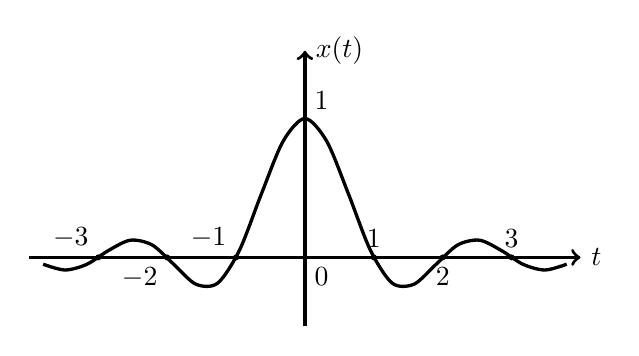
\begin{tikzpicture}[scale=1.75]
    \draw[->,very thick](0,-0.5)--(0,1.5)node[right]{$x(t)$};
    \draw[->,very thick](-2,0)--(2,0)node[right]{$t$};
    \draw[-,very thick]plot[smooth, domain=-1.9:1.9](\x,{1/(2*pi*\x)*sin(2*pi*\x r)});
    \node[above right]at(0,1){$1$};
    \node[above]at(0.5,0){$1$};
    \node[below]at(1,0){$2$};
    \node[above]at(1.5,0){$3$};
    \node[above left]at(-0.5,0){$-1$};
    \node[below left]at(-1,0){$-2$};
    \node[above left]at(-1.5,0){$-3$};
    \node[below right]at(0,0){$0$};
    \filldraw[black](0.5,0)circle(0.5pt);
    \filldraw[black](1,0)circle(0.5pt);
    \filldraw[black](1.5,0)circle(0.5pt);
    \filldraw[black](-0.5,0)circle(0.5pt);
    \filldraw[black](-1,0)circle(0.5pt);
    \filldraw[black](-1.5,0)circle(0.5pt);
\end{tikzpicture}
\end{document}